\documentclass[lettersize,journal]{IEEEtran}
\usepackage{amsmath,amsfonts}
\usepackage{algorithmic}
\usepackage{algorithm}
\usepackage{array}
\usepackage[caption=false,font=normalsize,labelfont=sf,textfont=sf]{subfig}
\usepackage{textcomp}
\usepackage{stfloats}
\usepackage{url}
\usepackage{verbatim}
\usepackage{graphicx}
\usepackage{cite}
\hyphenation{op-tical net-works semi-conduc-tor IEEE-Xplore}
% updated with editorial comments 8/9/2021

\begin{document}

\title{TwinPrompt: Dual-View Time-Series Prompting for Few-Shot Generative Classification}

\author{Shizhuo Deng,~\IEEEmembership{Member,~IEEE},
        Yonghui Qin,
        Boqian Lin,
        Dongyue Chen,
        and Tong Jia,~\IEEEmembership{Member,~IEEE}
        % <-this % stops a space
\thanks{This work was supported in part by the National Key R\&D Program of China under Grant 2024YFB4710900, in part by the Guangdong Basic and Applied Basic Research Foundation under Grant 2024A1515010244, in part by the National Natural Science Foundation of China under Grant U25A20477, and in part by the 111 Project under Grant B16009. (Corresponding authors: Dongyue Chen and Xinde Li.)}%
\thanks{Shizhuo Deng and Dongyue Chen are with the College of Information Science and Engineering, Key Laboratory of Data Analytics and Optimization for Smart Industry, Northeastern University, Shenyang 110819, China, and also with the Foshan Graduate School of Innovation, Northeastern University, Foshan 528311, China (e-mail: dengshizhuo@mail.neu.edu.cn; chendongyue@ise.neu.edu.cn).}%
\thanks{Yonghui Qin, Boqian Lin, and Tong Jia are with the College of Information Science and Engineering, Northeastern University, Shenyang 110819, China (e-mail: 2400885@stu.neu.edu.cn; lin.boqian@foxmail.com; jiatong@ise.neu.edu.cn).}}% <- 3. 调整顺序：将第2、3、5作的介绍提到第6作之前

% The paper headers
\markboth{Journal of \LaTeX\ Class Files,~Vol.~14, No.~8, August~2021}%
{Shell \MakeLowercase{\textit{et al.}}: A Sample Article Using IEEEtran.cls for IEEE Journals}

%\IEEEpubid{0000--0000/00\$00.00~\copyright~2021 IEEE}
% Remember, if you use this you must call \IEEEpubidadjcol in the second
% column for its text to clear the IEEEpubid mark.

\maketitle

\begin{abstract}
Few-shot time series classification (TSC) remains challenging because, under extremely limited supervision, a model must not only extract stable class-discriminative patterns from a handful of labeled examples, but also develop a decision mechanism that generalizes to unseen classes. Existing methods typically model time series from a single view, making it difficult to jointly capture local-to-global temporal dependencies and holistic waveform morphology. Meanwhile, although pretrained large language models (LLMs) offer strong conditional generative priors, their effective use in TSC is hindered by the representation gap between continuous-valued time series and the hidden space of language models. Moreover, if prediction is still performed with a conventional discriminative classification head, the generative decision-making capability of LLMs—aligned with their pretraining objective—cannot be fully exploited. To address these issues, we propose a unified generative framework for few-shot TSC. Our method first employs a dual-view time-series encoder, where a temporal branch and a visual branch extract complementary dynamic dependencies and morphological structure patterns, respectively. The resulting representations are then aligned to the hidden space of a frozen LLM through alignment pretraining. Finally, we reformulate classification as constrained generation of class-specific tokens, enabling the model to leverage the conditional generation capability of the LLM for few-shot decision-making, while constrained decoding further reduces prediction uncertainty in low-data regimes. Experiments under a strict few-shot protocol on UCR benchmarks show that the proposed method consistently outperforms existing deep learning baselines across multiple shot settings. Ablation studies further confirm the complementarity of the dual-view design, the stable gains and faster convergence brought by alignment pretraining, and the critical role of constrained decoding in generative few-shot classification.
\end{abstract}

\begin{IEEEkeywords}
Time-Series Classification, Few-Shot Learning, Generative Classification, Large Language Models, Prompting
\end{IEEEkeywords}

\section{Introduction}
Time series classification (TSC) is a core problem in machine learning, underpinning applications such as healthcare monitoring, industrial diagnosis, human activity recognition, and scientific sensing \cite{ismail2019deep}. While deep neural networks have substantially advanced fully supervised TSC, their success typically depends on having sufficiently many labeled sequences\cite{pan2024review}. In many practical settings, however, annotations are scarce, costly, or slow to acquire—for example in rare fault diagnosis, patient-specific monitoring, and newly deployed sensing systems. Few-shot TSC therefore remains a practically important and fundamentally difficult regime: the model must infer class-discriminative structure from only a handful of labeled examples per class while remaining robust to large intra-class variation and cross-domain heterogeneity\cite{tang2020interpretable}.

Existing few-shot TSC methods have mainly explored meta-learning, prototype- or shapelet-based reasoning, and spectral or contrastive representation learning \cite{barreda2024cosco,tang2020interpretable,yang2022spectral}. In parallel, recent work has begun to connect pretrained large language models (LLMs) to time-series analysis through quantization, projection, prompt-based adaptation, and multimodal interfaces \cite{zhang2024large,jin2024time,cheng2024advancing}. Yet these two lines have not fully met where few-shot TSC is hardest. Current LLM-based pipelines often rely on a single representation pathway, even though recent work increasingly suggests that visualized time-series signals can expose morphology-aware cues that are complementary to sequence-space modeling \cite{ni2025harnessing,liu2025picture}. They also face a persistent modality gap between continuous temporal features and the hidden space of frozen language models \cite{chang2025llm4ts,cheng2024advancing}. Moreover, final decisions are frequently made either by external discriminative heads or by unconstrained open-vocabulary generation, both of which are only weakly aligned with the autoregressive objective that causal LLMs are pretrained to solve.

We take the view that effective few-shot TSC with frozen causal LLMs is bottlenecked by three coupled issues: representation, alignment, and decision. First, under extreme label scarcity, a single-view encoder may fail to recover all class-discriminative cues from the input sequence. Second, even strong temporal features are of limited use unless they can be mapped into a latent interface that the frozen LLM can reliably exploit. Third, if the prediction mechanism is mismatched with autoregressive next-token generation, the model may underuse the time-series information already encoded in its internal states. Recent evidence that prompt outputs can substantially underestimate the time-series classification capability contained in LLM representations further reinforces this point \cite{schumacher2026prompting}.

Motivated by this perspective, we propose a dual-view generative framework for few-shot TSC. A patch-based temporal encoder, inspired by patchified time-series Transformers \cite{nietime}, captures local-to-global temporal dependencies directly in sequence space. In parallel, a visual branch renders each time series as a 2D image and extracts morphology-aware representations that emphasize waveform shape, texture, periodic structure, and spatialized anomalies. Rather than collapsing the two views prematurely, we preserve their token-level outputs and concatenate them before projection, so that the downstream model can condition jointly on temporal dynamics and morphological structure.

To make this dual-view evidence usable by a frozen causal LLM, we project the concatenated temporal tokens into the LLM hidden space and treat them as soft prompt tokens inserted into an instruction-style input. We further adopt a stage-wise alignment strategy before few-shot supervision. The first stage learns to produce LLM-compatible time-series representations and reduces the modality gap between temporal features and language-model hidden states. The second stage performs joint optimization of the dual-view encoder, the projection module, and lightweight LoRA adapters while keeping the main LLM backbone frozen. This design makes alignment a primary training target rather than an incidental by-product of few-shot finetuning, which is especially important when only a small support set is available. 

Finally, instead of attaching an external classifier, we reformulate few-shot TSC as constrained label-token generation. We introduce class-specific tokens into the tokenizer and train the model to generate the correct label token conditioned on textual instructions and dual-view time-series soft prompts. During inference, decoding is restricted to the candidate class tokens in the current episode together with the end-of-sequence token. This preserves consistency with the causal LLM’s native generation objective while removing irrelevant vocabulary degrees of freedom, thereby yielding more stable decisions under few-shot uncertainty.

Extensive experiments under a strict support/query protocol validate this formulation. Across shot settings, the dual-view model consistently outperforms either single branch alone; stage-wise alignment pretraining accelerates convergence, stabilizes optimization, and improves final accuracy; constrained decoding materially boosts prediction quality; and the overall framework surpasses strong deep-learning baselines at the same shot level. These results suggest that the key to few-shot TSC is not simply introducing a larger pretrained model, but enabling the model to see richer temporal evidence, align that evidence with a frozen LLM in latent space, and decide through a generation mechanism tailored to the episode label set.

In summary, our contributions are threefold: (1) we introduce a dual-view encoder that couples patch-based temporal modeling with morphology-aware visual modeling for few-shot TSC; (2) we present a stage-wise time-series-to-LLM alignment scheme with parameter-efficient adaptation for frozen causal LLMs; and (3) we cast few-shot TSC as constrained label-token generation and show that dual-view encoding, alignment pretraining, and constrained decoding each make measurable contributions to performance.

\section{Related Work}
\paragraph{Few-shot time series classification.}
Few-shot time series classification (TSC) has mainly been studied through meta-learning, metric learning, and prototype-based inductive biases. Narwariya et al.~\cite{narwariya2020meta} introduced a meta-learning framework that trains residual networks across heterogeneous UCR tasks for rapid adaptation under scarce supervision. Tang et al.~\cite{tang2020interpretable} proposed Dual Prototypical Shapelet Networks (DPSN), which combine representative class prototypes with discriminative local shapelets to improve both interpretability and data efficiency. Yang et al.~\cite{yang2022spectral} further explored spectral relations and introduced the Spectral Propagation Graph Network (SPGN) to propagate class information through spectrum-wise comparisons. More recently, COSCO~\cite{barreda2024cosco} improved few-shot multivariate TSC from the optimization perspective by combining sharpness-aware minimization with a prototypical loss. These methods demonstrate the importance of transferable priors and structured inductive biases, but they remain essentially discriminative pipelines and mostly operate within a single temporal representation space.

\paragraph{LLMs and foundation models for time series.}
Recent surveys show that foundation-model research for time series has rapidly expanded from adapting pretrained language models to building native temporal foundation models~\cite{jiang2024empowering,ye2024survey,shi2025large}. Representative adaptation-based approaches include TEST~\cite{sun2023test}, which aligns time-series embeddings with the LLM embedding space through text-prototype-aware contrastive learning; Time-LLM~\cite{jin2024time}, which reprograms time-series patches into a frozen LLM via text prototypes and prompt-as-prefix; and S$^2$IP-LLM~\cite{pan2024s}, which aligns time-series embeddings with semantic anchors derived from pretrained word embeddings. LLM4TS~\cite{chang2025llm4ts} further adopts a two-stage alignment-and-task fine-tuning strategy, while OpenTSLM~\cite{langer2025opentslm} moves toward native time-series language models with soft-prompt and cross-attention interfaces. A recent line of work has also begun to study few-shot classification with LLM-based architectures. The closest to our setting is LLMFew~\cite{chen2025large}, which uses a patch-wise temporal encoder, LoRA-tuned decoder, and a conventional classification head for few-shot multivariate TSC. Compared with this line, we focus on dual-view temporal evidence, explicit stage-wise alignment before few-shot adaptation, and generative label-token prediction rather than an external classifier. We are also motivated by recent ablation studies suggesting that naively attaching time-series inputs to pretrained LLMs is insufficient unless the temporal interface is meaningfully designed and aligned~\cite{tan2024language}.

\paragraph{Vision-based representations for time series.}
Beyond sequence-space modeling, a growing body of work represents time series as images so that waveform morphology, texture, periodicity, and holistic structural patterns can be captured by vision backbones. Recent surveys identify this as an increasingly important branch of time-series foundation modeling~\cite{ni2025harnessing}. In the context of multimodal reasoning, Liu et al.~\cite{liu2025picture} show that visualization can substantially improve LLM reasoning over time series. For classification, TiViT~\cite{roschmann2025time} demonstrates that pretrained vision transformers applied to imaged time series can yield highly competitive representations and are complementary to time-series foundation models. These results suggest that visualized signals expose discriminative cues that are not fully captured by sequence-only modeling. However, existing visual approaches are typically used as alternatives to temporal encoders or as interfaces for reasoning, rather than being fused at the token level with a temporal branch for few-shot generative classification.

\paragraph{Generative classification and constrained decoding.}
Casting classification as generation has been widely explored in NLP, most notably in the text-to-text paradigm of T5~\cite{raffel2020exploring}. Rather than relying on an external discriminative head, this paradigm formulates prediction as conditional token generation, making the decision process more naturally aligned with the pretrained objective of language models. In parallel, constrained decoding has been studied as a general mechanism for restricting generation to valid outputs under lexical or structural constraints~\cite{hokamp2017lexically,koo2024automata}. Inspired by these ideas, we formulate few-shot time series classification as generation of class-specific label tokens conditioned on textual instructions and time-series soft prompts. Instead of attaching a separate classifier, our model performs prediction in the native autoregressive manner of a frozen causal LLM, while restricting decoding to the candidate label space of the current episode further reduces irrelevant output freedom and improves decision stability under low-data uncertainty.

In summary, our method lies at the intersection of these four lines of work: few-shot TSC, LLM-based time-series adaptation, vision-based time-series representation learning, and generative classification with constrained decoding. It differs from prior work by jointly combining dual-view token-level encoding, stage-wise time-series-to-LLM alignment, and episode-wise constrained label-token generation in a unified framework for few-shot TSC.

\section{Method}

\subsection{Problem Setup}

We study few-shot time series classification (TSC) under an episodic setting.
Let $\mathcal{C}$ denote the label space of a dataset.
In each episode $e$, we sample a class subset $\mathcal{C}^{(e)} \subseteq \mathcal{C}$ and construct a support set
$\mathcal{S}^{(e)}=\{(x_i,y_i)\}_{i=1}^{N_s}$ and a query set
$\mathcal{Q}^{(e)}=\{(x_j,y_j)\}_{j=1}^{N_q}$ such that $y_i,y_j \in \mathcal{C}^{(e)}$.
Each input $x \in \mathbb{R}^{L}$ is a univariate time series of length $L$.
The goal is to predict the class label of each query example using only the limited labeled support examples in the current episode.

Instead of learning a conventional discriminative classifier, we reformulate few-shot TSC as \emph{constrained label-token generation}.
For each class $c \in \mathcal{C}$, we introduce a class-specific token $g_c$ into the tokenizer vocabulary.
Given an input time series and a textual instruction, the model is trained to generate the correct label token $g_y$ followed by an end-of-sequence token.
During inference, generation is restricted to the candidate label tokens in the current episode.
This turns few-shot TSC into conditional generation over an episode-specific label space.

\subsection{Framework Overview}

Our framework consists of four components:
(1) a dual-view time-series encoder,
(2) a lightweight projector that maps time-series features into the hidden space of a frozen causal LLM,
(3) a parameter-efficient adaptation module based on LoRA,
and (4) a generative decision layer implemented through class-specific token prediction.

Given a time series $x$, we encode it from two complementary views.
A temporal branch captures local-to-global temporal dependencies directly in sequence space, while a visual branch converts the series into a 2D image and extracts morphology-aware representations.
Unlike architectures that aggressively compress multimodal evidence into a small number of slots, we preserve the token-level outputs of both branches and directly concatenate them before projection.
The projected tokens are then injected into an instruction-style input as continuous soft prompts for a frozen causal LLM, which predicts a class token autoregressively.

\subsection{Dual-View Time-Series Encoder}

\paragraph{Temporal branch.}
We first partition the input series $x$ into overlapping patches of length $P$ with stride $S$,
yielding $M_t$ temporal patches:
\[
\mathbf{p}_m = x_{(m-1)S+1:(m-1)S+P}, \qquad m=1,\dots,M_t.
\]
Each patch is linearly embedded and augmented with positional information, and the resulting patch sequence is fed into a Transformer encoder:
\[
\mathbf{H}^{t} = F_t(\mathbf{p}_1,\dots,\mathbf{p}_{M_t}) \in \mathbb{R}^{M_t \times d_{ts}},
\]
where $F_t$ denotes the temporal encoder and $d_{ts}$ is the time-series feature dimension.
This branch is designed to model short-range local patterns, long-range dependencies, and temporal evolution dynamics in the original 1D signal space.

\paragraph{Visual branch.}
In parallel, we transform the same time series into a 2D visual representation:
\[
\mathbf{I} = \mathcal{R}(x),
\]
where $\mathcal{R}(\cdot)$ is a deterministic rendering function that converts the 1D signal into an image.
The rendered image is processed by a visual backbone $F_v$, producing a sequence of visual tokens:
\[
\widetilde{\mathbf{H}}^{v} = F_v(\mathbf{I}) \in \mathbb{R}^{M_v \times d_v}.
\]
Because the visual backbone and the temporal branch may operate in different feature spaces, we project the visual tokens into the same time-series feature dimension:
\[
\mathbf{H}^{v} = \widetilde{\mathbf{H}}^{v}\mathbf{W}_v + \mathbf{b}_v \in \mathbb{R}^{M_v \times d_{ts}}.
\]
This branch emphasizes morphology-aware cues such as waveform shape, periodic structure, texture-like patterns, and spatialized anomalies that may be less explicit in a purely sequential representation.

\paragraph{Token-level fusion.}
The two views are fused by direct concatenation at the token level:
\[
\mathbf{H} = [\mathbf{H}^{t}; \mathbf{H}^{v}] \in \mathbb{R}^{(M_t+M_v)\times d_{ts}}.
\]
Importantly, we do not apply slot-based pooling or early aggregation before fusion.
This preserves fine-grained evidence from both views and allows the downstream LLM to attend jointly to temporal dynamics and morphology-aware structure.

\subsection{Time-Series-to-LLM Interface}

The dual-view encoder outputs are not converted into textualized numbers.
Instead, they are mapped into the hidden space of a causal LLM through a lightweight projector:
\[
\mathbf{Z} = \mathbf{H}\mathbf{W}_p + \mathbf{b}_p \in \mathbb{R}^{M \times d_{llm}},
\]
where $M=M_t+M_v$ and $d_{llm}$ is the hidden size of the LLM.

We then build an instruction-style input for each sample.
The textual part contains:
(1) a task instruction stating that the problem is an $N$-class classification task and that the model should output only a class token,
(2) a short description specifying the time-series modality and length information,
and (3) a suffix prompt that asks for the answer.
Let $\mathbf{E}_{pre}$, $\mathbf{E}_{desc}$, and $\mathbf{E}_{suf}$ denote the corresponding text embeddings produced by the tokenizer and embedding layer of the LLM.
The final conditioning sequence is assembled as
\[
\mathbf{C}(x) = [\mathbf{E}_{pre}; \mathbf{E}_{desc}; \mathbf{Z}; \mathbf{E}_{suf}].
\]
Hence, the LLM receives a mixed sequence composed of text tokens and continuous time-series soft prompts.

\subsection{Generative Classification with Class Tokens}

For each class $c$, we add a unique label token $g_c$ to the tokenizer.
Given an example $(x,y)$, the target answer sequence is
\[
\mathbf{a}(y) = [g_y, \texttt{<eos>}].
\]
During training, the answer embeddings are appended to the conditioning sequence:
\[
\mathbf{X}(x,y) = [\mathbf{C}(x); \mathbf{E}(g_y); \mathbf{E}(\texttt{<eos>})].
\]
The model is optimized with an autoregressive language-modeling objective, but the loss is computed only on the answer segment:
\[
\mathcal{L}_{gen}
=
- \log p_\Theta(g_y \mid \mathbf{C}(x))
- \log p_\Theta(\texttt{<eos>} \mid \mathbf{C}(x), g_y).
\]
Therefore, the textual prompt and the time-series soft prompts serve purely as conditions, while supervision is concentrated on the generated label token and the end token.

In practice, we allow the token embedding matrix and the LM head to be trainable for implementation simplicity.
However, because supervision is applied only to the answer segment, the optimization pressure is primarily focused on the class-specific tokens and their surrounding decision interface.

\subsection{Constrained Decoding}

At inference time, the target answer is not appended.
Given the conditioning sequence $\mathbf{C}(x)$, the model generates at most two tokens.
To reduce irrelevant output freedom, decoding is constrained to the episode-specific candidate set
\[
\mathcal{V}^{(e)} = \{ g_c \mid c \in \mathcal{C}^{(e)} \} \cup \{\texttt{<eos>}\}.
\]
Because each class is represented by a single token, prediction is equivalent to
\[
\hat{y}
=
\arg\max_{c \in \mathcal{C}^{(e)}}
p_\Theta(g_c \mid \mathbf{C}(x)).
\]
The model then emits \texttt{<eos>} after the selected class token.
This constrained decoding strategy preserves consistency with the autoregressive objective while removing irrelevant open-vocabulary alternatives, leading to more stable decisions in low-data regimes.

\subsection{Stage-wise Alignment and Parameter-Efficient Adaptation}

A central challenge in our framework is the representation mismatch between time-series features and the latent space of the frozen LLM.
To address this issue, we adopt a stage-wise optimization strategy.

\paragraph{Stage 1: alignment warm-up.}
In the first stage, we optimize the dual-view encoder and the projector while keeping the main LLM backbone frozen and without activating LoRA.
This stage focuses on learning an LLM-compatible interface for the injected time-series tokens and stabilizes cross-modal alignment before joint adaptation.

\paragraph{Stage 2: joint adaptation.}
In the second stage, we continue training from the warm-up initialization and activate LoRA modules in the LLM.
The trainable parameters then include the dual-view encoder, the projector, the LoRA parameters, and the class-token-related embedding/output parameters, while the original LLM backbone remains frozen.
This design preserves the pretrained generative prior of the LLM while allowing parameter-efficient task adaptation.

When alignment pretraining is used, the same stage-wise schedule is first applied on the pretraining data to initialize the time-series-to-LLM interface, and the resulting weights are then adapted to downstream few-shot episodes.
When alignment pretraining is disabled, the model is trained directly on the downstream task using the same generative objective.

\subsection{Few-Shot Episodic Adaptation}

For few-shot learning, training is conducted only on the support set of each episode.
We consider both all-way $K$-shot episodes and $N$-way $K$-shot episodes.
For the latter, we first sample $N$ classes and then sample up to $K$ support examples per class.
If a class contains fewer than $K$ training examples, we use all available examples of that class rather than dropping it.
The query set is formed from test samples belonging to the same episode-specific class subset $\mathcal{C}^{(e)}$.

This protocol makes each run a self-contained episode with its own support set, query set, and decoding label space.
The final model is evaluated directly on the query set of the same episode, ensuring that both supervision and constrained decoding are matched to the current few-shot task.

\subsection{Full-Supervised Variant}

The same architecture also supports a full-supervised training regime.
This variant can be obtained by removing episodic sampling, training on the full training split, and performing constrained decoding over the complete dataset label space.
Therefore, the difference between the few-shot and full-supervised settings lies in the training protocol rather than in the model architecture itself.
\section{Other Resources}
See \cite{ref1,ref2,ref3,ref4,ref5} for resources on formatting math into text and additional help in working with \LaTeX .

\section{Text}
For some of the remainer of this sample we will use dummy text to fill out paragraphs rather than use live text that may violate a copyright.

Itam, que ipiti sum dem velit la sum et dionet quatibus apitet voloritet audam, qui aliciant voloreicid quaspe volorem ut maximusandit faccum conemporerum aut ellatur, nobis arcimus.
Fugit odi ut pliquia incitium latum que cusapere perit molupta eaquaeria quod ut optatem poreiur? Quiaerr ovitior suntiant litio bearciur?

Onseque sequaes rectur autate minullore nusae nestiberum, sum voluptatio. Et ratem sequiam quaspername nos rem repudandae volum consequis nos eium aut as molupta tectum ulparumquam ut maximillesti consequas quas inctia cum volectinusa porrum unt eius cusaest exeritatur? Nias es enist fugit pa vollum reium essusam nist et pa aceaqui quo elibusdandis deligendus que nullaci lloreri bla que sa coreriam explacc atiumquos simolorpore, non prehendunt lam que occum\cite{ref6} si aut aut maximus eliaeruntia dia sequiamenime natem sendae ipidemp orehend uciisi omnienetus most verum, ommolendi omnimus, est, veni aut ipsa volendelist mo conserum volores estisciis recessi nveles ut poressitatur sitiis ex endi diti volum dolupta aut aut odi as eatquo cullabo remquis toreptum et des accus dolende pores sequas dolores tinust quas expel moditae ne sum quiatis nis endipie nihilis etum fugiae audi dia quiasit quibus.
\IEEEpubidadjcol
Ibus el et quatemo luptatque doluptaest et pe volent rem ipidusa eribus utem venimolorae dera qui acea quam etur aceruptat.
Gias anis doluptaspic tem et aliquis alique inctiuntiur?

Sedigent, si aligend elibuscid ut et ium volo tem eictore pellore ritatus ut ut ullatus in con con pere nos ab ium di tem aliqui od magnit repta volectur suntio. Nam isquiante doluptis essit, ut eos suntionsecto debitiur sum ea ipitiis adipit, oditiore, a dolorerempos aut harum ius, atquat.

Rum rem ditinti sciendunti volupiciendi sequiae nonsect oreniatur, volores sition ressimil inus solut ea volum harumqui to see\eqref{deqn_ex1a} mint aut quat eos explis ad quodi debis deliqui aspel earcius.

\begin{equation}
\label{deqn_ex1a}
x = \sum_{i=0}^{n} 2{i} Q.
\end{equation}

Alis nime volorempera perferi sitio denim repudae pre ducilit atatet volecte ssimillorae dolore, ut pel ipsa nonsequiam in re nus maiost et que dolor sunt eturita tibusanis eatent a aut et dio blaudit reptibu scipitem liquia consequodi od unto ipsae. Et enitia vel et experferum quiat harum sa net faccae dolut voloria nem. Bus ut labo. Ita eum repraer rovitia samendit aut et volupta tecupti busant omni quiae porro que nossimodic temquis anto blacita conse nis am, que ereperum eumquam quaescil imenisci quae magnimos recus ilibeaque cum etum iliate prae parumquatemo blaceaquiam quundia dit apienditem rerit re eici quaes eos sinvers pelecabo. Namendignis as exerupit aut magnim ium illabor roratecte plic tem res apiscipsam et vernat untur a deliquaest que non cus eat ea dolupiducim fugiam volum hil ius dolo eaquis sitis aut landesto quo corerest et auditaquas ditae voloribus, qui optaspis exero cusa am, ut plibus.


\section{Some Common Elements}
\subsection{Sections and Subsections}
Enumeration of section headings is desirable, but not required. When numbered, please be consistent throughout the article, that is, all headings and all levels of section headings in the article should be enumerated. Primary headings are designated with Roman numerals, secondary with capital letters, tertiary with Arabic numbers; and quaternary with lowercase letters. Reference and Acknowledgment headings are unlike all other section headings in text. They are never enumerated. They are simply primary headings without labels, regardless of whether the other headings in the article are enumerated. 

\subsection{Citations to the Bibliography}
The coding for the citations is made with the \LaTeX\ $\backslash${\tt{cite}} command. 
This will display as: see \cite{ref1}.

For multiple citations code as follows: {\tt{$\backslash$cite\{ref1,ref2,ref3\}}}
 which will produce \cite{ref1,ref2,ref3}. For reference ranges that are not consecutive code as {\tt{$\backslash$cite\{ref1,ref2,ref3,ref9\}}} which will produce  \cite{ref1,ref2,ref3,ref9}

\subsection{Lists}
In this section, we will consider three types of lists: simple unnumbered, numbered, and bulleted. There have been many options added to IEEEtran to enhance the creation of lists. If your lists are more complex than those shown below, please refer to the original ``IEEEtran\_HOWTO.pdf'' for additional options.\\

\subsubsection*{\bf A plain  unnumbered list}
\begin{list}{}{}
\item{bare\_jrnl.tex}
\item{bare\_conf.tex}
\item{bare\_jrnl\_compsoc.tex}
\item{bare\_conf\_compsoc.tex}
\item{bare\_jrnl\_comsoc.tex}
\end{list}

\subsubsection*{\bf A simple numbered list}
\begin{enumerate}
\item{bare\_jrnl.tex}
\item{bare\_conf.tex}
\item{bare\_jrnl\_compsoc.tex}
\item{bare\_conf\_compsoc.tex}
\item{bare\_jrnl\_comsoc.tex}
\end{enumerate}

\subsubsection*{\bf A simple bulleted list}
\begin{itemize}
\item{bare\_jrnl.tex}
\item{bare\_conf.tex}
\item{bare\_jrnl\_compsoc.tex}
\item{bare\_conf\_compsoc.tex}
\item{bare\_jrnl\_comsoc.tex}
\end{itemize}


\subsection{Figures}
Fig. 1 is an example of a floating figure using the graphicx package.
 Note that $\backslash${\tt{label}} must occur AFTER (or within) $\backslash${\tt{caption}}.
 For figures, $\backslash${\tt{caption}} should occur after the $\backslash${\tt{includegraphics}}.


Fig. 2(a) and 2(b) is an example of a double column floating figure using two subfigures.
 (The subfig.sty package must be loaded for this to work.)
 The subfigure $\backslash${\tt{label}} commands are set within each subfloat command,
 and the $\backslash${\tt{label}} for the overall figure must come after $\backslash${\tt{caption}}.
 $\backslash${\tt{hfil}} is used as a separator to get equal spacing.
 The combined width of all the parts of the figure should do not exceed the text width or a line break will occur.
%
\begin{figure*}[!t]
\centering
\subfloat[]{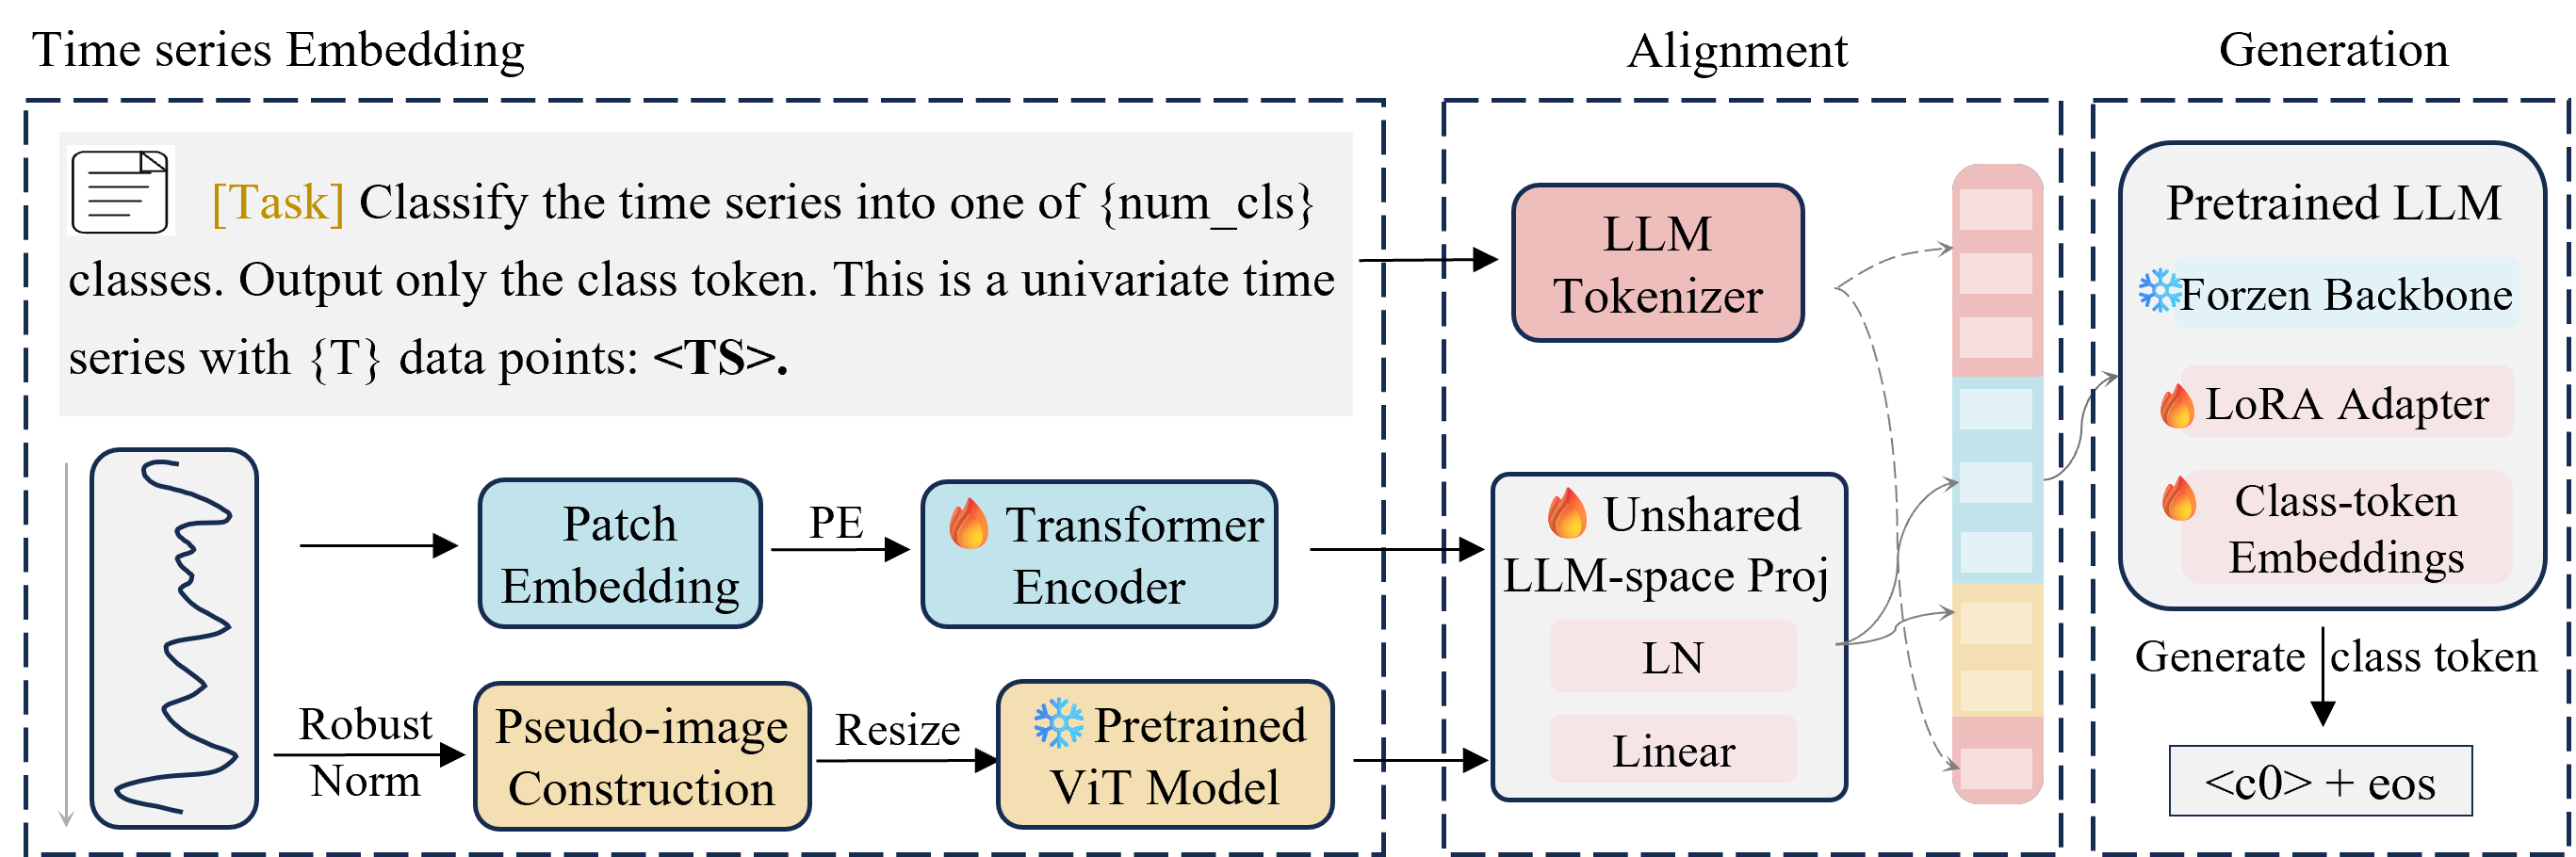
\includegraphics[width=2.5in]{fig/fig1.png}%
\label{fig_first_case}}
\hfil
\subfloat[]{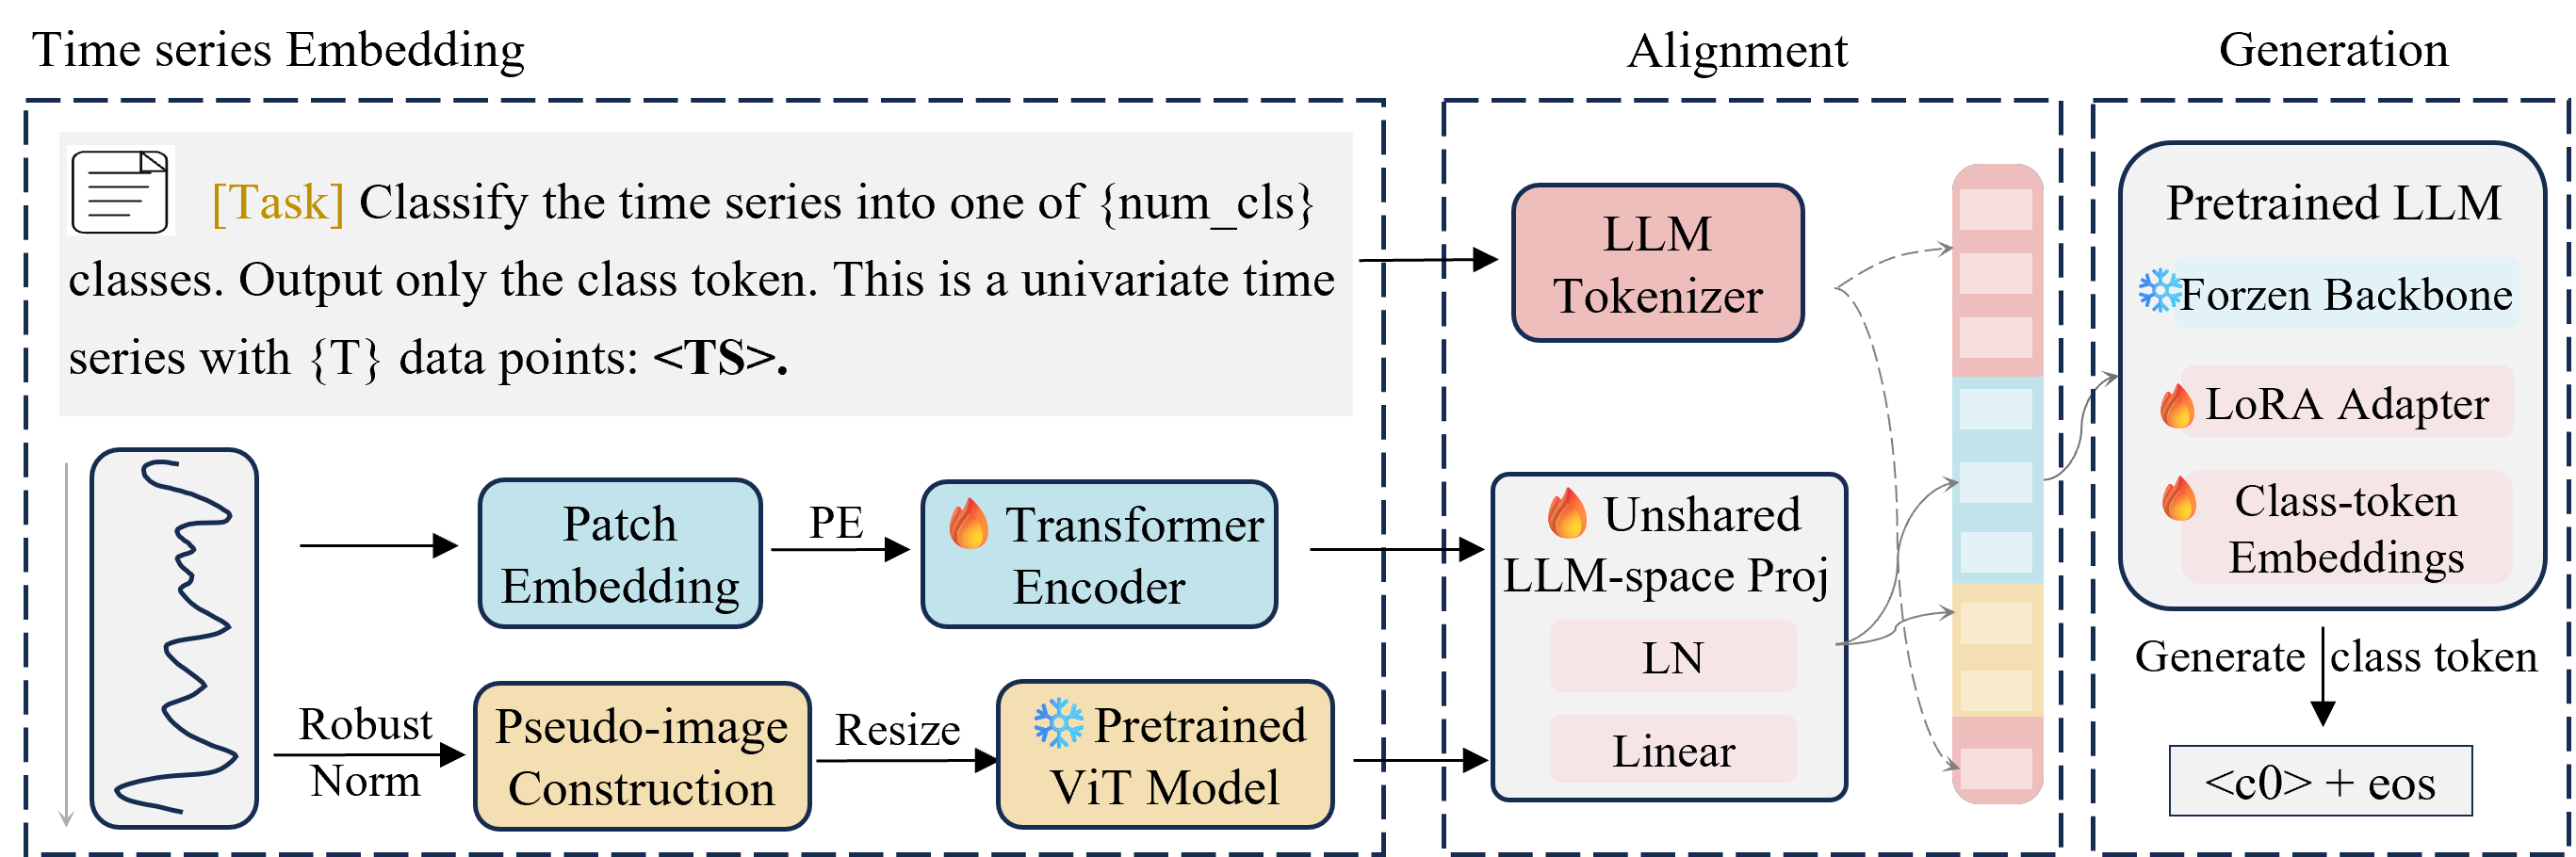
\includegraphics[width=2.5in]{fig/fig1.png}%
\label{fig_second_case}}
\caption{Dae. Ad quatur autat ut porepel itemoles dolor autem fuga. Bus quia con nessunti as remo di quatus non perum que nimus. (a) Case I. (b) Case II.}
\label{fig_sim}
\end{figure*}

Note that often IEEE papers with multi-part figures do not place the labels within the image itself (using the optional argument to $\backslash${\tt{subfloat}}[]), but instead will
 reference/describe all of them (a), (b), etc., within the main caption.
 Be aware that for subfig.sty to generate the (a), (b), etc., subfigure
 labels, the optional argument to $\backslash${\tt{subfloat}} must be present. If a
 subcaption is not desired, leave its contents blank,
 e.g.,$\backslash${\tt{subfloat}}[].


 

\section{Tables}
Note that, for IEEE-style tables, the
 $\backslash${\tt{caption}} command should come BEFORE the table. Table captions use title case. Articles (a, an, the), coordinating conjunctions (and, but, for, or, nor), and most short prepositions are lowercase unless they are the first or last word. Table text will default to $\backslash${\tt{footnotesize}} as
 the IEEE normally uses this smaller font for tables.
 The $\backslash${\tt{label}} must come after $\backslash${\tt{caption}} as always.
 
\begin{table}[!t]
\caption{An Example of a Table\label{tab:table1}}
\centering
\begin{tabular}{|c||c|}
\hline
One & Two\\
\hline
Three & Four\\
\hline
\end{tabular}
\end{table}

\section{Algorithms}
Algorithms should be numbered and include a short title. They are set off from the text with rules above and below the title and after the last line.

\begin{algorithm}[H]
\caption{Weighted Tanimoto ELM.}\label{alg:alg1}
\begin{algorithmic}
\STATE 
\STATE {\textsc{TRAIN}}$(\mathbf{X} \mathbf{T})$
\STATE \hspace{0.5cm}$ \textbf{select randomly } W \subset \mathbf{X}  $
\STATE \hspace{0.5cm}$ N_\mathbf{t} \gets | \{ i : \mathbf{t}_i = \mathbf{t} \} | $ \textbf{ for } $ \mathbf{t}= -1,+1 $
\STATE \hspace{0.5cm}$ B_i \gets \sqrt{ \textsc{max}(N_{-1},N_{+1}) / N_{\mathbf{t}_i} } $ \textbf{ for } $ i = 1,...,N $
\STATE \hspace{0.5cm}$ \hat{\mathbf{H}} \gets  B \cdot (\mathbf{X}^T\textbf{W})/( \mathbb{1}\mathbf{X} + \mathbb{1}\textbf{W} - \mathbf{X}^T\textbf{W} ) $
\STATE \hspace{0.5cm}$ \beta \gets \left ( I/C + \hat{\mathbf{H}}^T\hat{\mathbf{H}} \right )^{-1}(\hat{\mathbf{H}}^T B\cdot \mathbf{T})  $
\STATE \hspace{0.5cm}\textbf{return}  $\textbf{W},  \beta $
\STATE 
\STATE {\textsc{PREDICT}}$(\mathbf{X} )$
\STATE \hspace{0.5cm}$ \mathbf{H} \gets  (\mathbf{X}^T\textbf{W} )/( \mathbb{1}\mathbf{X}  + \mathbb{1}\textbf{W}- \mathbf{X}^T\textbf{W}  ) $
\STATE \hspace{0.5cm}\textbf{return}  $\textsc{sign}( \mathbf{H} \beta )$
\end{algorithmic}
\label{alg1}
\end{algorithm}

Que sunt eum lam eos si dic to estist, culluptium quid qui nestrum nobis reiumquiatur minimus minctem. Ro moluptat fuga. Itatquiam ut laborpo rersped exceres vollandi repudaerem. Ulparci sunt, qui doluptaquis sumquia ndestiu sapient iorepella sunti veribus. Ro moluptat fuga. Itatquiam ut laborpo rersped exceres vollandi repudaerem. 
\section{Mathematical Typography \\ and Why It Matters}

Typographical conventions for mathematical formulas have been developed to {\bf provide uniformity and clarity of presentation across mathematical texts}. This enables the readers of those texts to both understand the author's ideas and to grasp new concepts quickly. While software such as \LaTeX \ and MathType\textsuperscript{\textregistered} can produce aesthetically pleasing math when used properly, it is also very easy to misuse the software, potentially resulting in incorrect math display.

IEEE aims to provide authors with the proper guidance on mathematical typesetting style and assist them in writing the best possible article. As such, IEEE has assembled a set of examples of good and bad mathematical typesetting \cite{ref1,ref2,ref3,ref4,ref5}. 

Further examples can be found at \url{http://journals.ieeeauthorcenter.ieee.org/wp-content/uploads/sites/7/IEEE-Math-Typesetting-Guide-for-LaTeX-Users.pdf}

\subsection{Display Equations}
The simple display equation example shown below uses the ``equation'' environment. To number the equations, use the $\backslash${\tt{label}} macro to create an identifier for the equation. LaTeX will automatically number the equation for you.
\begin{equation}
\label{deqn_ex1}
x = \sum_{i=0}^{n} 2{i} Q.
\end{equation}

\noindent is coded as follows:
\begin{verbatim}
\begin{equation}
\label{deqn_ex1}
x = \sum_{i=0}^{n} 2{i} Q.
\end{equation}
\end{verbatim}

To reference this equation in the text use the $\backslash${\tt{ref}} macro. 
Please see (\ref{deqn_ex1})\\
\noindent is coded as follows:
\begin{verbatim}
Please see (\ref{deqn_ex1})\end{verbatim}

\subsection{Equation Numbering}
{\bf{Consecutive Numbering:}} Equations within an article are numbered consecutively from the beginning of the
article to the end, i.e., (1), (2), (3), (4), (5), etc. Do not use roman numerals or section numbers for equation numbering.

\noindent {\bf{Appendix Equations:}} The continuation of consecutively numbered equations is best in the Appendix, but numbering
 as (A1), (A2), etc., is permissible.\\

\noindent {\bf{Hyphens and Periods}}: Hyphens and periods should not be used in equation numbers, i.e., use (1a) rather than
(1-a) and (2a) rather than (2.a) for subequations. This should be consistent throughout the article.

\subsection{Multi-Line Equations and Alignment}
Here we show several examples of multi-line equations and proper alignments.

\noindent {\bf{A single equation that must break over multiple lines due to length with no specific alignment.}}
\begin{multline}
\text{The first line of this example}\\
\text{The second line of this example}\\
\text{The third line of this example}
\end{multline}

\noindent is coded as:
\begin{verbatim}
\begin{multline}
\text{The first line of this example}\\
\text{The second line of this example}\\
\text{The third line of this example}
\end{multline}
\end{verbatim}

\noindent {\bf{A single equation with multiple lines aligned at the = signs}}
\begin{align}
a &= c+d \\
b &= e+f
\end{align}
\noindent is coded as:
\begin{verbatim}
\begin{align}
a &= c+d \\
b &= e+f
\end{align}
\end{verbatim}

The {\tt{align}} environment can align on multiple  points as shown in the following example:
\begin{align}
x &= y & X & =Y & a &=bc\\
x' &= y' & X' &=Y' &a' &=bz
\end{align}
\noindent is coded as:
\begin{verbatim}
\begin{align}
x &= y & X & =Y & a &=bc\\
x' &= y' & X' &=Y' &a' &=bz
\end{align}
\end{verbatim}





\subsection{Subnumbering}
The amsmath package provides a {\tt{subequations}} environment to facilitate subnumbering. An example:

\begin{subequations}\label{eq:2}
\begin{align}
f&=g \label{eq:2A}\\
f' &=g' \label{eq:2B}\\
\mathcal{L}f &= \mathcal{L}g \label{eq:2c}
\end{align}
\end{subequations}

\noindent is coded as:
\begin{verbatim}
\begin{subequations}\label{eq:2}
\begin{align}
f&=g \label{eq:2A}\\
f' &=g' \label{eq:2B}\\
\mathcal{L}f &= \mathcal{L}g \label{eq:2c}
\end{align}
\end{subequations}

\end{verbatim}

\subsection{Matrices}
There are several useful matrix environments that can save you some keystrokes. See the example coding below and the output.

\noindent {\bf{A simple matrix:}}
\begin{equation}
\begin{matrix}  0 &  1 \\ 
1 &  0 \end{matrix}
\end{equation}
is coded as:
\begin{verbatim}
\begin{equation}
\begin{matrix}  0 &  1 \\ 
1 &  0 \end{matrix}
\end{equation}
\end{verbatim}

\noindent {\bf{A matrix with parenthesis}}
\begin{equation}
\begin{pmatrix} 0 & -i \\
 i &  0 \end{pmatrix}
\end{equation}
is coded as:
\begin{verbatim}
\begin{equation}
\begin{pmatrix} 0 & -i \\
 i &  0 \end{pmatrix}
\end{equation}
\end{verbatim}

\noindent {\bf{A matrix with square brackets}}
\begin{equation}
\begin{bmatrix} 0 & -1 \\ 
1 &  0 \end{bmatrix}
\end{equation}
is coded as:
\begin{verbatim}
\begin{equation}
\begin{bmatrix} 0 & -1 \\ 
1 &  0 \end{bmatrix}
\end{equation}
\end{verbatim}

\noindent {\bf{A matrix with curly braces}}
\begin{equation}
\begin{Bmatrix} 1 &  0 \\ 
0 & -1 \end{Bmatrix}
\end{equation}
is coded as:
\begin{verbatim}
\begin{equation}
\begin{Bmatrix} 1 &  0 \\ 
0 & -1 \end{Bmatrix}
\end{equation}\end{verbatim}

\noindent {\bf{A matrix with single verticals}}
\begin{equation}
\begin{vmatrix} a &  b \\ 
c &  d \end{vmatrix}
\end{equation}
is coded as:
\begin{verbatim}
\begin{equation}
\begin{vmatrix} a &  b \\ 
c &  d \end{vmatrix}
\end{equation}\end{verbatim}

\noindent {\bf{A matrix with double verticals}}
\begin{equation}
\begin{Vmatrix} i &  0 \\ 
0 & -i \end{Vmatrix}
\end{equation}
is coded as:
\begin{verbatim}
\begin{equation}
\begin{Vmatrix} i &  0 \\ 
0 & -i \end{Vmatrix}
\end{equation}\end{verbatim}

\subsection{Arrays}
The {\tt{array}} environment allows you some options for matrix-like equations. You will have to manually key the fences, but there are other options for alignment of the columns and for setting horizontal and vertical rules. The argument to {\tt{array}} controls alignment and placement of vertical rules.

A simple array
\begin{equation}
\left(
\begin{array}{cccc}
a+b+c & uv & x-y & 27\\
a+b & u+v & z & 134
\end{array}\right)
\end{equation}
is coded as:
\begin{verbatim}
\begin{equation}
\left(
\begin{array}{cccc}
a+b+c & uv & x-y & 27\\
a+b & u+v & z & 134
\end{array} \right)
\end{equation}
\end{verbatim}

A slight variation on this to better align the numbers in the last column
\begin{equation}
\left(
\begin{array}{cccr}
a+b+c & uv & x-y & 27\\
a+b & u+v & z & 134
\end{array}\right)
\end{equation}
is coded as:
\begin{verbatim}
\begin{equation}
\left(
\begin{array}{cccr}
a+b+c & uv & x-y & 27\\
a+b & u+v & z & 134
\end{array} \right)
\end{equation}
\end{verbatim}

An array with vertical and horizontal rules
\begin{equation}
\left( \begin{array}{c|c|c|r}
a+b+c & uv & x-y & 27\\ \hline
a+b & u+v & z & 134
\end{array}\right)
\end{equation}
is coded as:
\begin{verbatim}
\begin{equation}
\left(
\begin{array}{c|c|c|r}
a+b+c & uv & x-y & 27\\
a+b & u+v & z & 134
\end{array} \right)
\end{equation}
\end{verbatim}
Note the argument now has the pipe "$\vert$" included to indicate the placement of the vertical rules.


\subsection{Cases Structures}
Many times cases can be miscoded using the wrong environment, i.e., {\tt{array}}. Using the {\tt{cases}} environment will save keystrokes (from not having to type the $\backslash${\tt{left}}$\backslash${\tt{lbrace}}) and automatically provide the correct column alignment.
\begin{equation*}
{z_m(t)} = \begin{cases}
1,&{\text{if}}\ {\beta }_m(t) \\ 
{0,}&{\text{otherwise.}} 
\end{cases}
\end{equation*}
\noindent is coded as follows:
\begin{verbatim}
\begin{equation*}
{z_m(t)} = 
\begin{cases}
1,&{\text{if}}\ {\beta }_m(t),\\ 
{0,}&{\text{otherwise.}} 
\end{cases}
\end{equation*}
\end{verbatim}
\noindent Note that the ``\&'' is used to mark the tabular alignment. This is important to get  proper column alignment. Do not use $\backslash${\tt{quad}} or other fixed spaces to try and align the columns. Also, note the use of the $\backslash${\tt{text}} macro for text elements such as ``if'' and ``otherwise.''

\subsection{Function Formatting in Equations}
Often, there is an easy way to properly format most common functions. Use of the $\backslash$ in front of the function name will in most cases, provide the correct formatting. When this does not work, the following example provides a solution using the $\backslash${\tt{text}} macro:

\begin{equation*} 
  d_{R}^{KM} = \underset {d_{l}^{KM}} {\text{arg min}} \{ d_{1}^{KM},\ldots,d_{6}^{KM}\}.
\end{equation*}

\noindent is coded as follows:
\begin{verbatim}
\begin{equation*} 
 d_{R}^{KM} = \underset {d_{l}^{KM}} 
 {\text{arg min}} \{ d_{1}^{KM},
 \ldots,d_{6}^{KM}\}.
\end{equation*}
\end{verbatim}

\subsection{ Text Acronyms Inside Equations}
This example shows where the acronym ``MSE" is coded using $\backslash${\tt{text\{\}}} to match how it appears in the text.

\begin{equation*}
 \text{MSE} = \frac {1}{n}\sum _{i=1}^{n}(Y_{i} - \hat {Y_{i}})^{2}
\end{equation*}

\begin{verbatim}
\begin{equation*}
 \text{MSE} = \frac {1}{n}\sum _{i=1}^{n}
(Y_{i} - \hat {Y_{i}})^{2}
\end{equation*}
\end{verbatim}

\section{Conclusion}
The conclusion goes here.


\section*{Acknowledgments}
This should be a simple paragraph before the References to thank those individuals and institutions who have supported your work on this article.



{\appendix[Proof of the Zonklar Equations]
Use $\backslash${\tt{appendix}} if you have a single appendix:
Do not use $\backslash${\tt{section}} anymore after $\backslash${\tt{appendix}}, only $\backslash${\tt{section*}}.
If you have multiple appendixes use $\backslash${\tt{appendices}} then use $\backslash${\tt{section}} to start each appendix.
You must declare a $\backslash${\tt{section}} before using any $\backslash${\tt{subsection}} or using $\backslash${\tt{label}} ($\backslash${\tt{appendices}} by itself
 starts a section numbered zero.)}



%{\appendices
%\section*{Proof of the First Zonklar Equation}
%Appendix one text goes here.
% You can choose not to have a title for an appendix if you want by leaving the argument blank
%\section*{Proof of the Second Zonklar Equation}
%Appendix two text goes here.}



\bibliographystyle{IEEEtran}
\bibliography{references}


\newpage

\section{Biography Section}
If you have an EPS/PDF photo (graphicx package needed), extra braces are
 needed around the contents of the optional argument to biography to prevent
 the LaTeX parser from getting confused when it sees the complicated
 $\backslash${\tt{includegraphics}} command within an optional argument. (You can create
 your own custom macro containing the $\backslash${\tt{includegraphics}} command to make things
 simpler here.)
 
\vspace{11pt}

\bf{If you include a photo:}\vspace{-33pt}
\begin{IEEEbiography}[{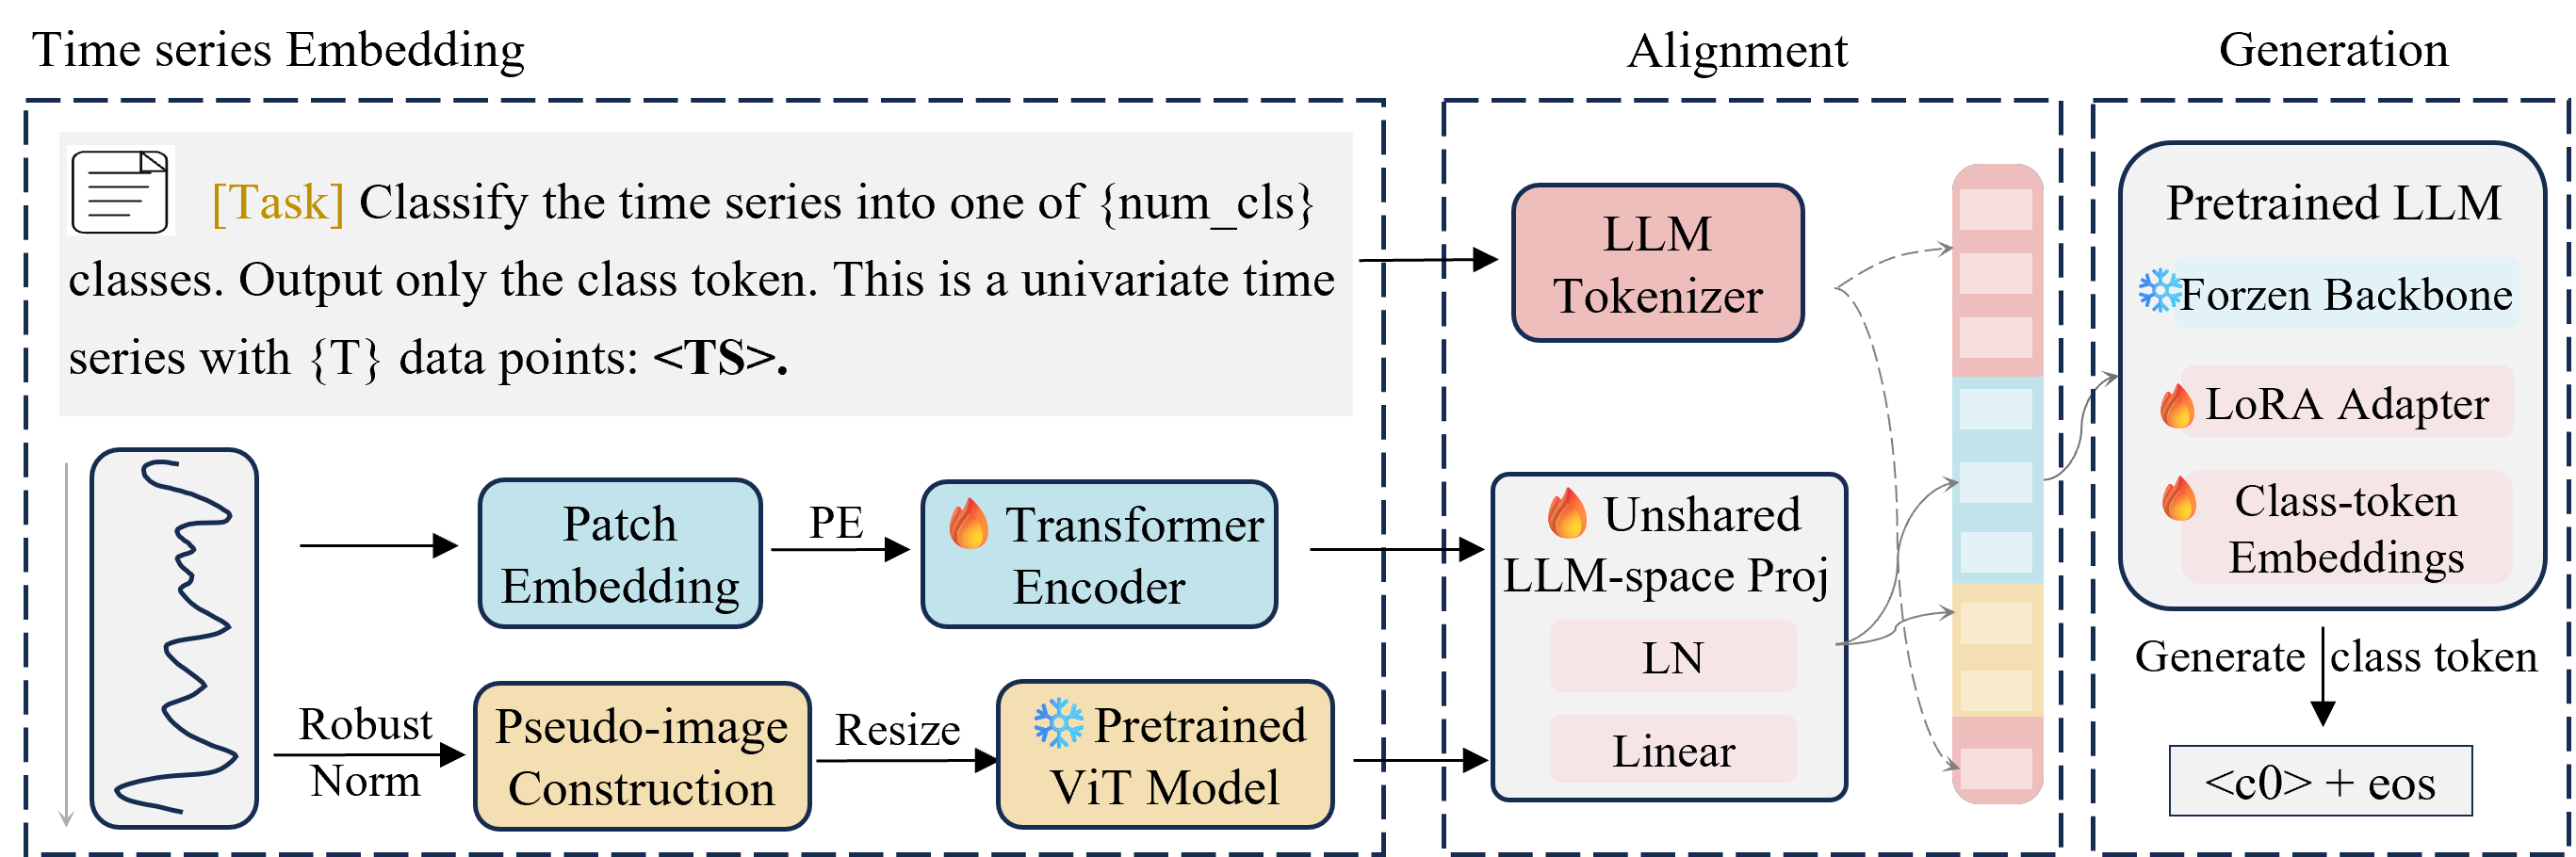
\includegraphics[width=1in,height=1.25in,clip,keepaspectratio]{fig/fig1.png}}]{Michael Shell}
Use $\backslash${\tt{begin\{IEEEbiography\}}} and then for the 1st argument use $\backslash${\tt{includegraphics}} to declare and link the author photo.
Use the author name as the 3rd argument followed by the biography text.
\end{IEEEbiography}

\vspace{11pt}

\bf{If you will not include a photo:}\vspace{-33pt}
\begin{IEEEbiographynophoto}{John Doe}
Use $\backslash${\tt{begin\{IEEEbiographynophoto\}}} and the author name as the argument followed by the biography text.
\end{IEEEbiographynophoto}




\vfill

\end{document}

